\documentclass[conference]{IEEEtran}
\usepackage{blindtext, graphicx, algpseudocode, float, color, amsmath}


% correct bad hyphenation here
\hyphenation{op-tical net-works semi-conduc-tor com-plexi-ty}


\begin{document}

\title{An Improvement of Controlling Quality of \\Large Scale Water-Level Data in Thailand}

\author{\IEEEauthorblockN{Nuttapon Pattanavijit, Peerapon Vateekul}
\IEEEauthorblockA{
Department of Computer Engineering\\
Faculty of Engineering, Chulalongkorn University\\
Phayathai Road, Pathumwan\\
Bangkok, Thailand, 10330\\
Email: {nuttapon.p@student.chula.ac.th, peerapon.v@chula.ac.th}
}
\and
\IEEEauthorblockN{Kanoksri Sarinnapakorn}
\IEEEauthorblockA{
Hydro and Agro Informatics Institute\\
Ministry of Science and Technology\\
Thailand, 10400\\
Email: kanoksri@haii.or.th
}}

% make the title area
\maketitle


\begin{abstract}
%\boldmath
Extremely change in precipitation level such as water level can cause severe damage. In order to acknowledge changes, Hydro and Agro Informatics Institute has installed telemetry system across Thailand to collect and analyze precipitation level. However, to use its data in researching, incorrect data must be filtered. In previous work, we successfully detect various problems in water level data accurately. Still, outliers detection algorithm  and missing pattern algorithm proposed in the previous work still room for improvement in terms of running time and ease of implementation. One of problems is that both algorithms is relied on complicated clustering which is unnecessary. In this paper, we propose to improve the clustering algorithm used in the previous work for water-level data. A linear clustering algorithm is invented and used to replace the old clustering algorithm. As a result, we can speed up the outliers detection algorithm and hold the same running time on missing pattern algorithm but increase simplicity and ease of implementation. Moreover, compared with the previous work we measure actual running time of our algorithms and found that they significantly help reduce the running time.

\end{abstract}

\begin{IEEEkeywords}
\color{red} Do, not, forget, to, insert, keyword, here
\end{IEEEkeywords}

\IEEEpeerreviewmaketitle

\section{Introduction} \label{sec:intro}

Thailand has faced many dreadful climate-related disaster including floods, droughts, and tropical cyclones. They have happened year after year and cause severe loss. For example, In 2011, seasonal flooding results in US\$ 45.7 billion damage to Thailand’s economy, which is 1.1\% of the country’s GDP [1]. Also, the climate-related disaster bring difficulties to agriculture and industry, which are backbones of Thailand economy. To handle these disaster, the government established many organization to cooperatively counteract with it. One of the organization is Hydro and Agro Informatics Institute (HAII). HAII's main focus is to research and utilize knowledge in agricultural and water resource management to confront the climate disaster [2].

In order to conduct researches, they have collected precipitation data by installing telemetry systems across Thailand. The telemetry system is a device that is used to collect physical, chemical, and biological data from its various sensors [3]. For instance, river’s water level, rainfall level, humidity, and temperature can be measured. Currently, Hydro and Agro Informatics Institute (HAII) have already installed over 800 telemetry system across Thailand. Fig. \ref{fig:tele_station_map} shows example of location where telemetry systems were installed. Each system send data from its many sensors back to central database every 10 minutes via cellular network. And, all of the data is stored order by timestamp. From these numbers, we can estimate that there are 3.45 million records of data added to database every month. Since HAII have collected precipitation data for over 5 years, we can assume that we are dealing with approximately 207 million records.

\begin{figure}
	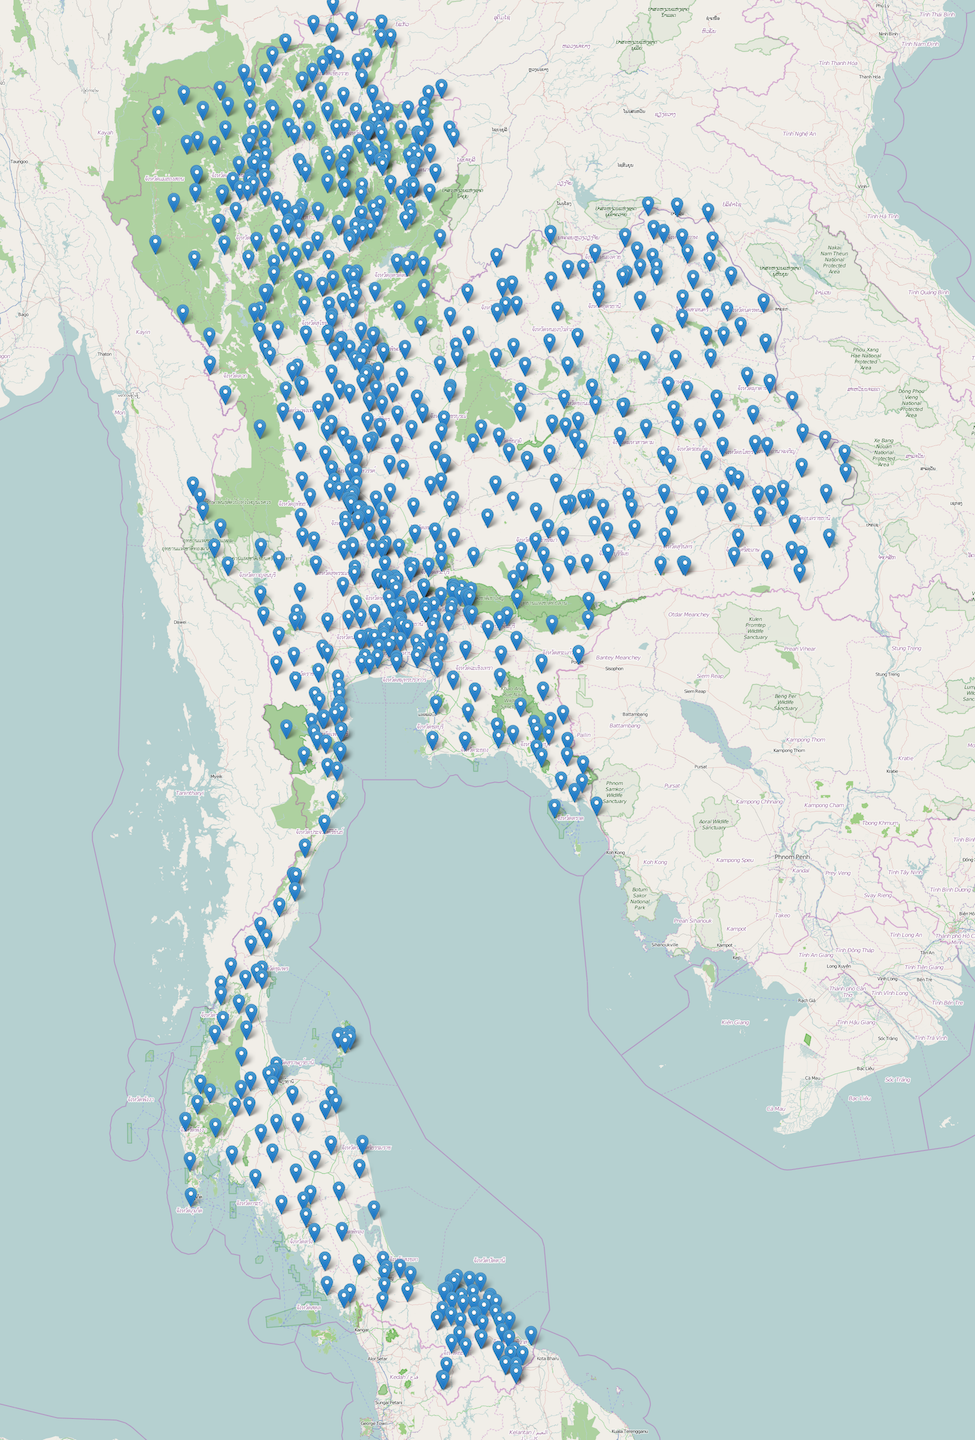
\includegraphics[width=\linewidth]{map.png}
	\caption{Map of Thailand indicates where telemetry system was installed.}
	\label{fig:tele_station_map}
\end{figure}

Sometimes, incorrect data is reported from the telemetry systems such as minus value of cumulative rainfall level, or river’s water level suddenly changed from one level to another, which are not possible. In addition, data loss can also be occurred due to poor cellular network in rural area. These inconsistent data is not suitable to be used in researches since it might lead to inaccurate results.

To filtered out incorrect data efficiently, our previous work [5] proposed algorithms to detect anomalies in water level data, which includes outliers, and missing pattern algorithm. Example of anomaly data detected by these algorithms is illustrated in Fig. \ref{fig:example_outliers}, and Fig. \ref{fig:example_missingpattern}. However, both outliers detection algorithms and missing pattern is heavily relied on clustering algorithm. \textit{DBSCAN} algorithm is used to do the clustering task. The \textit{DBSCAN} itself have $O(n\log{n})$ running time if it is implemented using special data structures that support region query such as \textit{R*-Tree} or \textit{k-d Tree}, which seem to be very complex, and it have $O(n^2)$ running time if no special data is used. This can cause outlier detection algorithm's running time rise up to $O(n\log{n})$ or $O(n^2)$, which is not quite suitable for over 200 million records of data. Moreover it unnecessarily add complication and time used in implementing both algorithms. Also, real runtime might be slow due to overhead of the algorithms.

In this paper, we proposed to improve the clustering algorithm in the previous work for water-level data. A linear clustering algorithm is invented and used to replace \textit{DBSCAN} clustering. The linear clustering algorithm helps improve both outliers detection algorithm and missing pattern algorithm for water-level data. As a result, the linear clustering algorithm helps increase speed and simplicity, yet maintain same accuracy of the algorithms. The outliers detection algorithm's running time is dwindled to $O(n)$. The missing pattern algorithm also achieves faster real running-time, even though holds the same theoretical running-time as previous work at $O(n\log{n})$.

\begin{figure}
	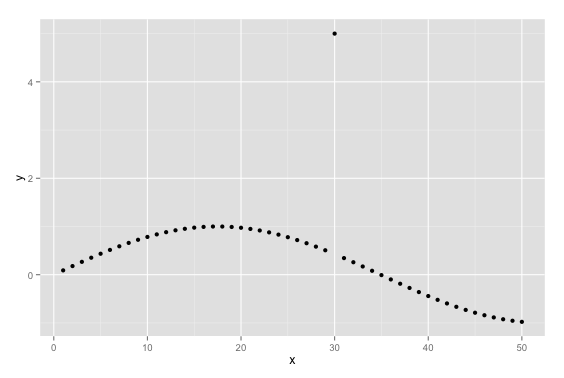
\includegraphics[width=\linewidth]{figure1.png}
	\caption{Example of data with outliers.}
	\label{fig:example_outliers}
\end{figure}

\begin{figure}
	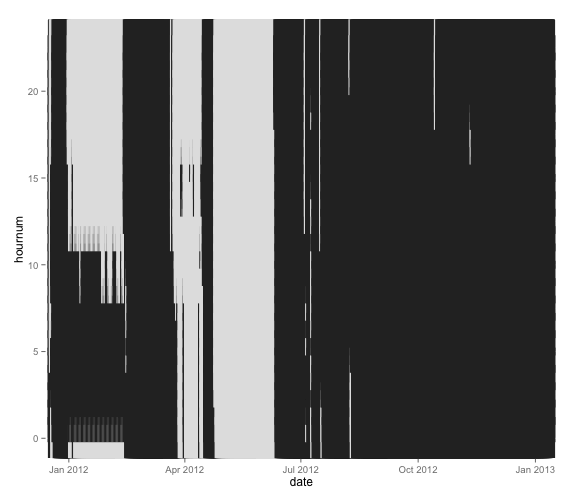
\includegraphics[width=\linewidth]{figure3.png}
	\caption{Example of data with missing pattern. X-axis represent date of the data. Y-axis indicate hour of day of the data. The lighter area shows date and hour where data was missing.}
	\label{fig:example_missingpattern}
\end{figure}

The paper is organized as follows. Section \ref{sec:previous} recaps our previous work and points out its running time. Our approach to refine the both algorithms are illustrated in Section \ref{sec:propose}. Experiment results are shown in Section \ref{sec:xperiments}. Last, Section \ref{sec:conclusion} delivers a conclusion.

\section{Previous Data Quality Management\\and Its Running Time} \label{sec:previous}

Our previous work proposed two algorithms to control quality of water-level data, outliers and missing pattern. Both of the algorithms apply clustering technique in order to detect anomaly data and pattern of data. DBSCAN was selected as a clustering algorithms. Note that for the time dimension, 10 minutes will be counted as a distance of 1 unit because data points is captured in 10 minutes interval and dataset is already sorted by timestamp.

In each subsection, since our previous previous work has not stated about the running time yet, we will brief each algorithm, illustrate its pseudocode, and analyze its running time in order to later refine both algorithms.

\subsection{Outliers Detection Algorithm}
In previous work, we detect outliers by directly applies \textit{DBSCAN} to water-level data. \textit{DBSCAN}'s required parameters, minimum number of points \textit{minpts} and distance epsilon \textit{eps}, is set to 3 and 1.05 respectively in order to classify data which have extreme difference in value compared to adjacent data as a noise. Fig. \ref{fig:outliers_pseudocode} illustrates pseudocode of outliers detection algorithm. $C$ is an array of cluster index. Data point $d_{i}$ is in $k$-th cluster if $C_{i} = k$ and $k \neq 0$. If $k = 0$, $d_{i}$ is considered as a noise. $N$ is an array storing index of noise data. If $C_{i} = 0$, then $i \in N$.

\begin{figure}
\begin{algorithmic}[1]
\Procedure{Detect-Outliers}{$d$}
\State $minpts\gets3$
\State $eps\gets1.05 $
\State $C\gets\emptyset$\Comment{Set of cluster of data index}
\State $N\gets\emptyset$\Comment{Set of noise data index}
\State $C, N \gets $\Call{DBSCAN}{$d, minpts, eps$}
\State \Return{$N$}
\EndProcedure
\end{algorithmic}
\caption{Pseudocode of outliers detection algorithm.}
\label{fig:outliers_pseudocode}
\end{figure}

From pseudocode in Fig. \ref{fig:outliers_pseudocode}, it is obvious that running time of \textsc{Detect-Outliers} is based on \textsc{DBSCAN}. Thus, we can conclude that \textsc{Detect-Outliers} complexity is $O(n^2)$ or $O(n\log{n})$ -- depends on the data structure inside \textsc{DBSCAN}.

\subsection{Missing Pattern Algorithm}

Proposed in previous work, missing pattern algorithm is used to detect pattern of missing data. There are many steps required in missing pattern algorithm. First, it convert water-level data into frequency domain, which count how many data is missing during each hour ($f_{0} ,f_{1}, \ldots, f_{23}$). Second, we use DBSCAN to analyze the frequency. If there are more than one cluster detected, there must be at least two hours having significantly different missing frequency $(f_{i})$. Then, we determine whether it contains missing pattern in overall data. Next, divided-and-conquer technique was applied to find missing pattern in subset of data. Last, we merge overlapped missing result together.

To be easier to explain, we rewrite its pseudocode from previous work in figure \ref{fig:missingpattern_pseudocode}. Result of \textsc{Missing-Pattern} procedure is returned as a list of tuples indicating start date and end date of pattern. Also, list is always sorted by start date of tuples.

\begin{figure}
\begin{algorithmic}[1]
\Procedure{Missing-Pattern}{$d$}
\If{$end - start \le \textit{minDataReq}$}
\State\Return{$\emptyset$}\Comment{Too few data}
\EndIf
\State $f \gets$ \Call{Hourly-Missing-Frequency}{$d$}
\State $minpts \gets 1$
\State $eps \gets \frac{|d|}{2}$
\State $C, N \gets$ \Call{DBSCAN}{$f, minpts, eps$}
\State $C' \gets \text{ array of all } C_{i} \neq 0$
\State $\textit{haveOverallMP} \gets \Call{Unique}{C'} \ge 2$ \Comment{at least 2 clusters}
\State
\State $P_{l} \gets $\Call{Missing-Pattern}{$d_{1} \ldots d_{\frac{|d|}{2}}$}
\State $P_{r} \gets$ \Call{Missing-Pattern}{$d_{\frac{|d|}{2}+1} \ldots d_{|d|}$}
\State $P \gets$ \Call{Combine-Result}{$P_{l}, P_{r}, \textit{haveOverallPattern}$}
\State
\State $\textit{mergeGap} \gets 15$ \Comment{15 days}
\State \Return{\Call{Merge-Overlap-Pattern}{$P, \textit{mergeGap}$}}
\EndProcedure
\end{algorithmic}
\caption{Pseudocode of missing pattern algorithm.}
\label{fig:missingpattern_pseudocode}
\end{figure}

From Fig. \ref{fig:missingpattern_pseudocode}, \textsc{Hourly-Missing-Frequency} on line 5 can be done in $O(|d|)$ by using counting sort with 24 bucket representing missing frequency of each hour of day ($f_{0},\ldots,f_{23}$). \textsc{Combine-Result} on line 14 is done in $O(1)$ by checking 8 possible cases. And, \textsc{Merge-Overlap-Pattern} could be executed in $O(|d|)$. Since the tuples in $P$ is sorted and not literally overlap, we can sequentially check each adjacent pair of tuples whether it should be merged. For the \textit{DBSCAN} in line 8, since $f$ always have 24 elements, the \textit{DBSCAN} always has $O(1)$ running time.

Since it uses divide-and-conquer, We can compute the complexity of by using \textit{master method}, which the complexity of algorithm can be represent in:

\[
T(n) = aT(\frac{n}{b}) + f(n)
\]

For missing pattern algorithm, $f(n)$ is equal to $O(n)$, which is the slowest running time in each recurrence. By applying \textit{master method}, running time of the algorithm is:

\[
\begin{array}{lcl}
T(n) & = & 2T(\frac{n}{2}) + O(n \log{n})\\
     & = & O(n \log{n})
\end{array}
\]

Even though the clustering algorithm is already has $O(1)$ running time, we think that using \textit{DBSCAN} for only 24 data points is unnecessary and contain huge overhead. Also, if we need to implement the \textit{DBSCAN} ourselves, it is too complicated to be use with only 24 data points.

\section{Proposed Improved Algorithms} \label{sec:propose}

Our proposed algorithms aim to solve the bottleneck in outliers detection algorithm and simplify the clustering in missing pattern algorithm. To do that, we try to create a new clustering algorithm which can imitate \textit{DBSCAN}'s result but with more efficiency, by using some facts about precipitation data and the algorithms themselves.

First, since the data was captured from a sensor, we can assume that at time $t$, there will be only one $d_{t}$. This fact implies that there is no need to search for adjacent points in two dimension.

Second, outliers algorithm and missing pattern algorithm produce best result when $\textit{minpts} = 3$ and $\textit{minpts} = 1$ respectively. Let $C$ be an array of cluster index. Data point $d_{i}$ is in $k$-th cluster if $C_{i} = k$ and $k \neq 0$. If $k = 0$, $d_{i}$ is considered as a noise. We can say that if $\textit{minpts} \le 3$, following properties are always true:

\begin{enumerate}
	\item if $C_{i} = k; k \neq 0$ (\textit{$k$}-th cluster) and $|d_{i+1} - d_{i}| \le \textit{eps}$, then $C_{i+1} = k$ too.
	\item $|\{i \mid C_{i} = k\}| \ge \textit{minpts}$ for all $k \ge 1$ 
\end{enumerate}

The first property shows that it is suffice to determine the cluster by measure distance between adjacent pair of data points. It is true because if $\textit{minpts} = 1$, at least $d_{i}$ can form its own cluster and add $d_{i+1}$ to its cluster. If $\textit{minpts} = 2$ and $C_{i} = k$, there must be another data point $j$ where $C_{j} = k, j < i$ within distance $\textit{eps}$. So $i$ can be add freely into $k$-th cluster ($C_{i} = k$). Last, if $\textit{minpts} = 3$, since $i$ is already in $C_{k}$, there must be another data point $j $ where $C_{j} = k, j < i$ within distance $\textit{eps}$. So, if $|d_{i+1} - d_{i}| \le \textit{eps}$, $d_{i}$ will satisfy $\textit{minpts} = 3$ (including itself) condition. Thus, $i+1$ can be added into $k$-th cluster.

The second property shows that every cluster must have at least \textit{minpts} data points. Assume that cluster $k$ is the smallest cluster possible, cluster $k$ must have at least one core data point in order to form a cluster. Let $d_{i}$ be the only core data point where $C_{i} = k$. $d_{i}$ must have at least $\textit{minpts}$ data point within distance $\textit{eps}$ (including itself). So, we can conclude that $|\{i \mid C_{i} = k\}| \ge \textit{minpts}$.

With this two properties, we can create an algorithm which can imitate \textit{DBSCAN}'s result for $\textit{minpts} \le 3$. Fig. \ref{fig:clustering_pseudocode} illustrates its pseudocode.

\begin{figure}
\begin{algorithmic}[1]
\Procedure{Linear-Cluster}{$d, minpts, eps$}
	\State $C_{tmp} \gets \emptyset$
	\State $C \gets \text{ array of size } |d|$
	\State $k \gets 0$
	\State $N \gets \emptyset$
%	\State $n_{C_{tmp}} \gets 0$
	\For{$i \gets 1 \text{ to } |d| + 1$}
		\State $newCluster \gets \text{false}$
		\If{$i = 1 \textbf{ or } i = |d|+1 \textbf{ or } |d_{i} - d_{i-1}| > eps$}
			\State $newCluster \gets \text{true}$
		\EndIf
		\If{$newCluster$ and $|C_{tmp}| \ge minpts$}
		    \State $k \gets k + 1$			    
			\State $C_{i} \gets k$ ; $\forall i \in C_{tmp}$
			\State $C_{tmp} \gets \emptyset$
		\ElsIf{$newCluster$}
			\State $C_{i} \gets 0$ ; $\forall i \in C_{tmp}$			
			\State $N \gets N \cup C_{tmp}$
			\State $C_{tmp} \gets \emptyset$
		\EndIf
		
		\State add $i$ to $C_{tmp}$ 
		
	\EndFor
	\State \Return{$C, N$}
\EndProcedure	
\end{algorithmic}
\caption{Pseudocode of new clustering algorithm.}
\label{fig:clustering_pseudocode}
\end{figure}

From Fig. \ref{fig:clustering_pseudocode}, the pseudocode work by following steps. First, it creates a temporary cluster an assume that $d_{i}$ is in cluster (start from $d_{1}$). Then, it checks the distance to its next adjacent data point ($d_{i+1}$). If the distance is less than $eps$, put $d_{i+1}$ in the same temporary cluster. Otherwise, create new temporary cluster and assume that $d_{i+1}$ is in it. Before creating new temporary cluster, we determine whether the previous temporary cluster can be formed into real cluster by counting data points inside it. If it has more than $minpts$ points, it can be formed as a real cluster. If not, all data point inside it should be considered as noise.

The \textsc{Linear-Cluster} algorithm has $O(n)$ running time even though it contains nested loop in line 6 and line 13 or 16. Since every $i$ will be a member of $C_{tmp}$ only once, line 13 and 16 will be executed only $n$ times in total. Thus, we can conclude that it has $O(n)$ running time.

Therefore, we can replace \textit{DBSCAN} in outliers algorithm and missing pattern algorithm with \textsc{Linear-Cluster} to reduce it's overall complexity. The outliers algorithm become $O(n)$ in complexity. For missing pattern, although the clustering process already has $O(1)$ running time, but \textsc{Linear-Cluster} is far more uncomplicated compare to \textsc{DBSCAN}. This helps reduce overhead in real running time and decrease implementation time for developers.


\section{Experiments} \label{sec:xperiments}

Lorem Ipsum

\section{Conclusion} \label{sec:conclusion}

Lorem Ipsum

\begin{thebibliography}{1}

\bibitem{IEEEhowto:kopka}
H.~Kopka and P.~W. Daly, \emph{A Guide to \LaTeX}, 3rd~ed.\hskip 1em plus
  0.5em minus 0.4em\relax Harlow, England: Addison-Wesley, 1999.

\end{thebibliography}

\end{document}


